\chapter{Sverdrup balance and basin-scale circulation}
\label{chap:sverdrup}

\includegraphics[width=6.5in]{figs/Geostrophic/HaidaEddy}

We saw above that the Ekman balance can drive convergences and divergences in the ocean, and that these cause the water to pile up preferentially creating pressure gradients.  The pressure gradients are then balanced by the Coriolis force, in the geostrophic balance, and water flows parallel to lines of constant pressure, clockwise around highs in the Northern hemisphere.  

This \emph{all} happens on the large scale.  If we consider the subtropical gyre, between 15 and 45 degrees, there is an Ekman convergence towards the centre of the gyre, and that causes there to be a sea-surface high there.  The water will flow around that sea-surface high in a clockwise direction (northern hemisphere).  However that leaves two questions:
\begin{enumerate}
    \item How strong will the flow be?  Alternately, how high will the highs in the middle of the gyre be?  
    \item Why is the gyre asymmetric east-west?  
\end{enumerate}

The answer is, as we will see below, that the flow is driven by the conservation of angular momentum acting in the presence of basin-scale changes in the Coriolis frequency.  Water with a negative (clockwise) torque exerted on it can either spin with negative (clockwise) angular momentum, or it can move to a region with lower background ``planetary'' angular momentum. 

\section{Circulation}

Idealizing the winds and seasurface in the subtropical gyre we have the idea that the winds blow from west to east in the westerlies (45 N) and east to west in the Trades (15 N; \fref{fig:GyreSketch}).  Based on the dynamics as we've understood them so far, this leads to an Ekman convergence everywhere in the gyre, and a raising of the seasurface height, and causing a downwelling.  

\begin{figure}[hbt]
  \begin{center}
    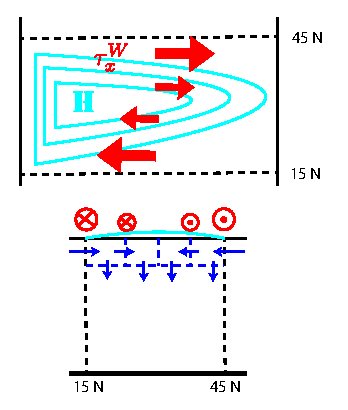
\includegraphics{figs/Sverdrup/GyreSketch}
    \caption{Idealized sketch of the wind stress in the subtropical gyre (northern hemisphere).   Top panel is from above, with coasts on the west and east side.  Westerlies peak at 45 N, and the trades at 15 N.  This makes a high in the middle, but offset to the west.  Bottom panel is the same situation looking at the side from the east towards the west. The Ekman layer is shown with the blue arrows, noting that there is downwelling throughout this gyre.}
    \label{fig:GyreSketch}  
  \end{center}
\end{figure}

However, the observed gyre is asymmetric, with the high concentrated near the western boundary. This implies that the velocity is largely equatorward everywhere in the gyre, except to the west of the high, along the \Wikiref{Western boundary}. The real situation is even more asymmetric than pictured in \fref{fig:GyreSketch}.  If we remember that the geostrophic interior velocity is proportional to the strength of the pressure gradient, then we would expect very slow flow towards the south in the interior, and very fast flow along this western boundary.  The western boundary current in the N. Pacific subtropical gyre is the \Wikiref{Kuroshio}; the \Wikiref{Gulf Stream} is the corresponding current in the Atlantic.  

\section{Conservation of potential vorticity}

The way to understand the gyre circulation is to consider the conservation of angular momentum, or in fluid mechanics we call it \Wikiref{potential vorticity}.  Just like any angular momentum, the potential vorticity changes in response to torque, in this case from the wind and seafloor.  A simplified version, useful for our case is:
\begin{equation}
    \frac{d}{dt}\left(\frac{\zeta + f}{H} \right) = \frac{1}{H^2\rho_0} \left[\frac{d\tau_y^W}{dx} - \frac{d\tau_x^W}{dy} + \frac{d\tau_y^B}{dx} - \frac{d\tau_x^B}{dy}\right]
\end{equation}
Here the term on the left side of the equation is the potential vorticity, and the term on the right side the torque due to the wind stress ($\tau_x^W, \tau_y^W$) and bottom friction ($\tau^B$).  $H$ is the water depth, and $f$ is the Coriolis parameter, which we keep in mind varies with latitude, or $y$.  We call this the \emph{planetary vorticity} and is the vertical angular momentum due to the earth's rotation.  
\begin{marginfigure}
    \includegraphics{figs/Sverdrup/relativevortsketch}
    \caption{Sketch of velocity gradients in a counter clockwise flow.  Note $\zeta>0$ in this flow.}
    \label{fig:relativevortsketch}  
\end{marginfigure}
The term $\zeta$ is the \Wikiref{relative vorticity} of the flow and is defined as:
\begin{equation}
    \zeta = \frac{dv}{dx} - \frac{du}{dy}
\end{equation}
where $u$ and $v$ are the x- and y-components of velocity.  It is relatively straight forward to see how this relates to a spinning flow (\fref{fig:relativevortsketch}).  Consider a flow spinning in a counter-clockwise manner.  The velocity gradients in such a flow are such that $zeta > 0$.  This uses the \Wikiref{right-hand rule}, which says that if you curl your right hand fingers in the direction of rotation, your thumb will point up for positive vorticity and down for negative vorticity (this is just a convention, and could have just as easily been the other way, but it is useful to choose one convention and stick with it).  Of course a clockwise flow has a negative vorticity.  

The same logic and sign convention applies to torque.  In the gyre sketched in \fref{fig:GyreSketch}, the gradients in $\tau^W$ are such that $\frac{d\tau_x^W}{dy} < 0$, so the wind is exerting a negative torque on the water.  


\begin{derivbox}[label={box:potentialvort}]{Derivation of potential vorticity}
Potential vorticity for a barotropic fluid is relatively straight forward to derive.  We  need the momentum equations and the continuity equation:
\begin{eqnarray*}
    \frac{du}{dt} & = & -\frac{1}{\rho}\frac{dP}{dx} + fv + \frac{1}{\rho}\frac{d\tau_x}{dz}\\
    \frac{dv}{dt} & = & -\frac{1}{\rho}\frac{dP}{dy} - fu + \frac{1}{\rho}\frac{d\tau_y}{dz}
\end{eqnarray*}
If we take $-d/dy$ of the first equation and $d/dx$ of the second and add them, then the pressure term drops out:
\begin{equation}
    \frac{d}{dt} \left( \frac{dv}{dx} - \frac{du}{dy}\right) = -f \left(\frac{du}{dx} + \frac{dv}{dy} \right) + \frac{1}{\rho}\left(\frac{d^2\tau_y}{dz\,dx} - \frac{d^2\tau_x}{dz\,dy}\right)
\end{equation}
and we note that the first term is just the derivative of $\zeta$ with time.  

We integrate this vertically from the sea-floor to sea surface, and assume that the water is $H$ deep, including any sea-surface displacements.   
\begin{equation}
    H\frac{d\zeta}{dt}  = -f H \left(\frac{du}{dx} + \frac{dv}{dy} \right) + \frac{1}{\rho}\left(\frac{d\tau_y^W}{dx} - \frac{d\tau_x^W}{dy}\right) + \frac{1}{\rho}\left(\frac{d\tau_y^B}{dx} - \frac{d\tau_x^B}{dy}\right) 
\end{equation}
So now we use the fact that $\frac{du}{dx} + \frac{dv}{dy} = -dW/dz = H^{-1}\frac{dH}{dt}$.  


\end{derivbox}


